\documentclass[11pt,a4paper]{article}
\usepackage[T1]{fontenc}
\usepackage{lmodern}
\usepackage{microtype}
\usepackage[margin=2.2cm]{geometry}
\usepackage{graphicx}
\usepackage{booktabs}
\usepackage{tabularx}
\usepackage{enumitem}
\usepackage{caption}
\usepackage{float}
\usepackage{needspace}
\usepackage{tikz}
\usetikzlibrary{positioning,arrows.meta}
\usepackage[hidelinks]{hyperref}

\setlist{itemsep=2pt,topsep=4pt}
\captionsetup{font=small,labelfont=bf}
\setlength{\parindent}{0pt}
\setlength{\parskip}{5pt}

\title{\textbf{Prohori: Progress Report}\\[4pt]\large OpenCV AI Competition 2026 --- AWS Compute Grant check-in}
\author{S.\,M.\ Hozaifa Hossain, team Prohori}
\date{20 October 2026}

\begin{document}
\maketitle
\vspace{-1.5em}

\section{Project}
Prohori measures concrete crack width in millimetres from a phone photo. The user places a printed ChArUco board next to the crack; OpenCV uses the board to correct for camera angle and scale and reports the width with an uncertainty range. When a photo cannot support a reliable measurement, the app tells the user how to retake it.

Live app: \url{https://184-194-241-186.sslip.io} (tap \emph{Demo samples} to try it without a board).

\section{Progress}
\begin{itemize}
  \item \textbf{Measurement pipeline:} ChArUco detection, \texttt{solvePnP} pose, rectification to a known px/mm, crack location, and per-crack width with uncertainty (about 1.5\,s per 12\,MP photo).
  \item \textbf{Quality gate:} a learned check, calibrated with conformal risk control, that certifies a width only when the photo supports it, and attaches a 90\% range to each width.
  \item \textbf{Capture agent:} after each photo, an Amazon Bedrock agent (Nova Lite) chooses the next step (accept, move closer, hold steadier, fix lighting, reposition the board, or stop) from OpenCV's measurements. A free rules policy is the default.
  \item \textbf{Phone web app, history and alerts:} per-joint visit history, change detection beyond measurement uncertainty, engineer alerts with an approval step, and automatic face blurring (OpenCV YuNet) before any photo is stored.
  \item \textbf{Testing:} 206 automated tests passing.
\end{itemize}

\begin{figure}[H]
  \centering
  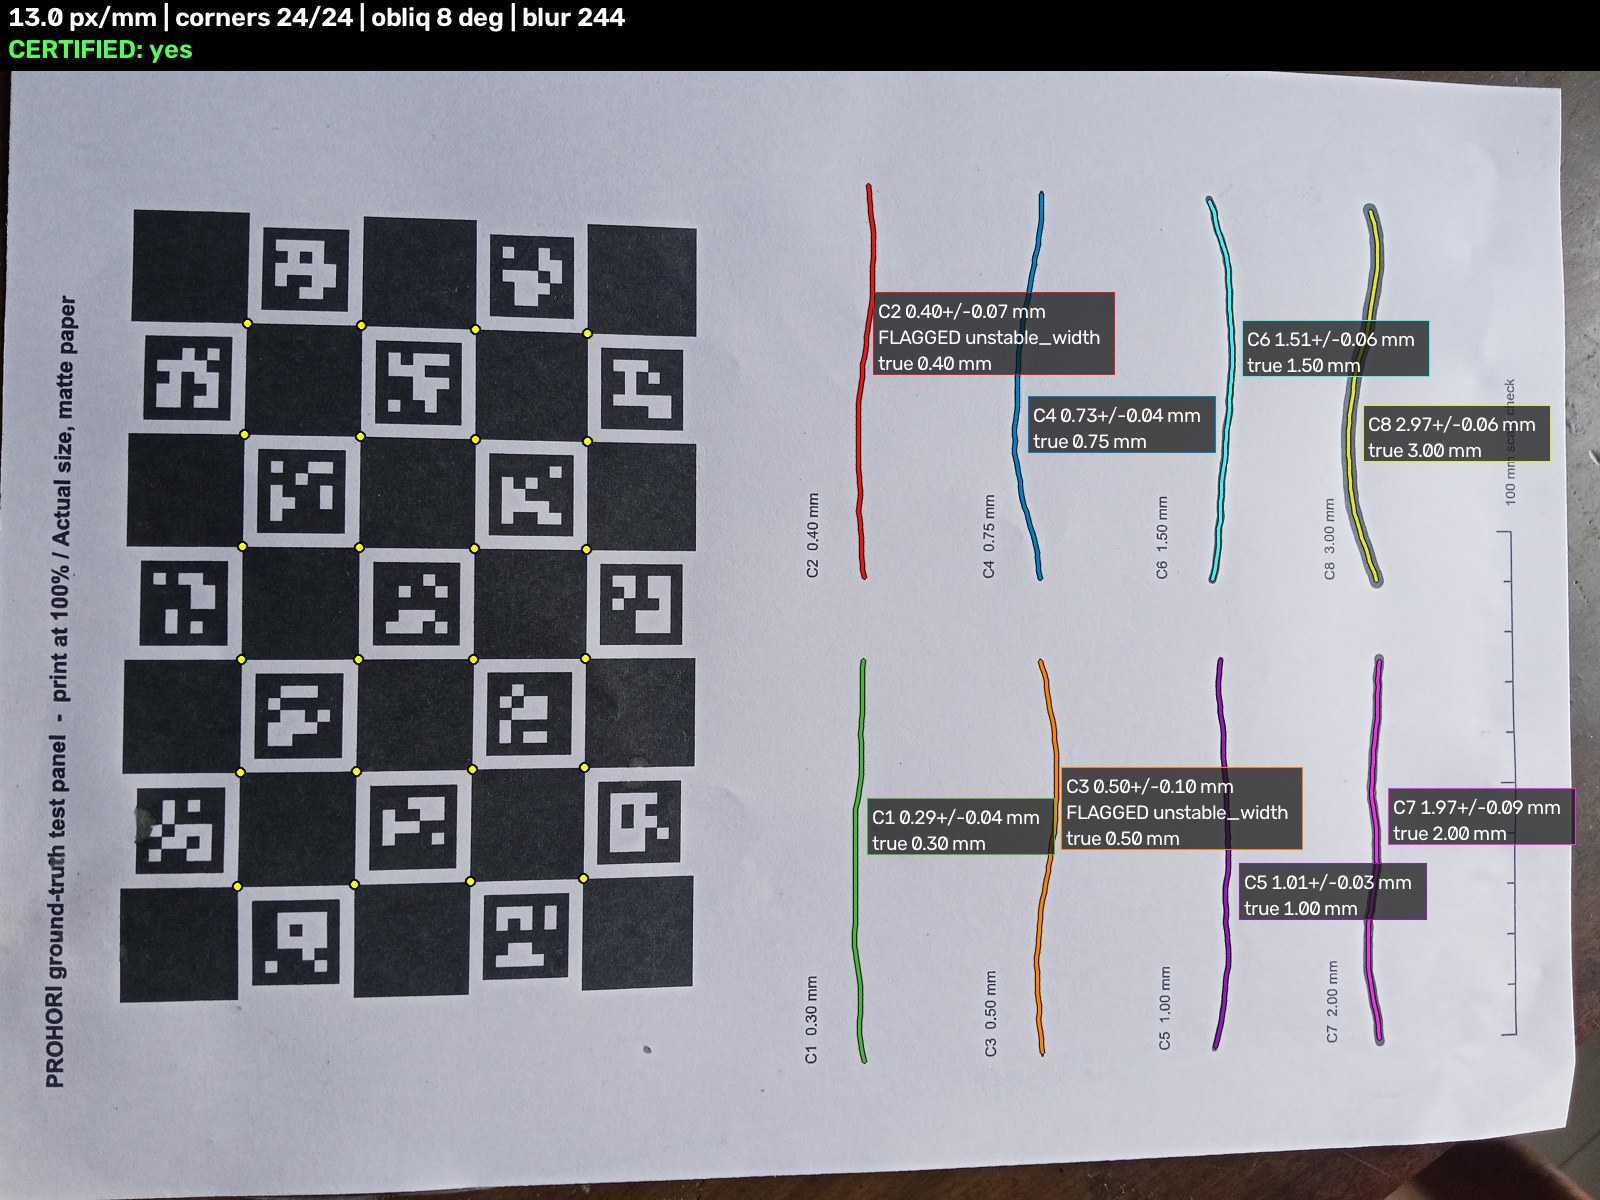
\includegraphics[width=0.62\textwidth]{img/overlay_best.jpg}
  \caption{A phone photo processed by Prohori. The board corners set the scale; each crack is labelled with its measured width next to the true printed width (e.g.\ 0.29\,mm vs 0.30, 1.01\,mm vs 1.00, 2.97\,mm vs 3.00).}
\end{figure}

\begin{figure}[H]
  \centering
  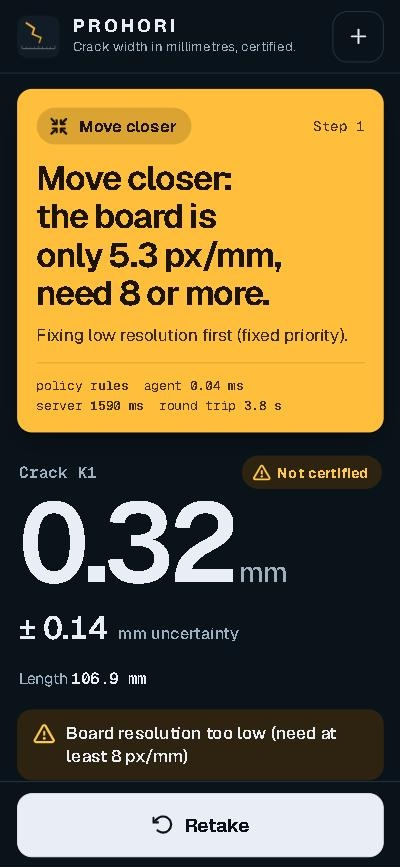
\includegraphics[width=0.235\textwidth]{img/crop_02_too_far_move_closer.jpg}\hfill
  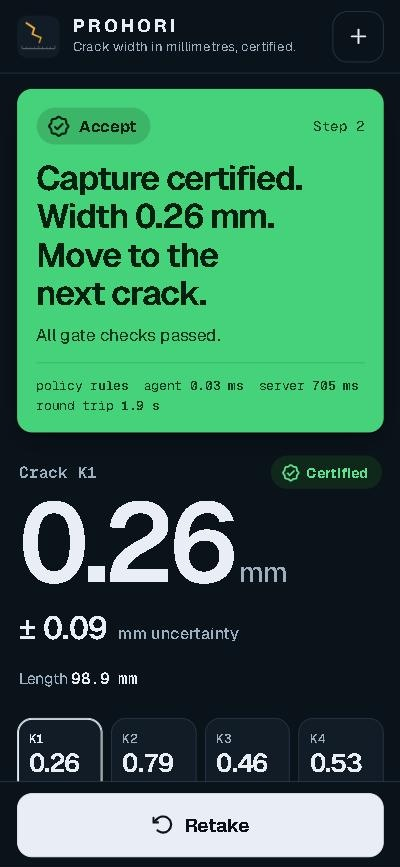
\includegraphics[width=0.235\textwidth]{img/crop_03_certified_accept.jpg}\hfill
  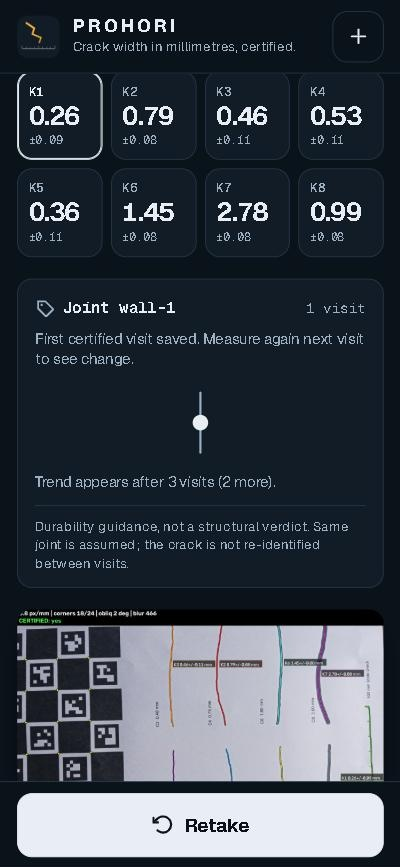
\includegraphics[width=0.235\textwidth]{img/crop_04_all_cracks_and_history.jpg}\hfill
  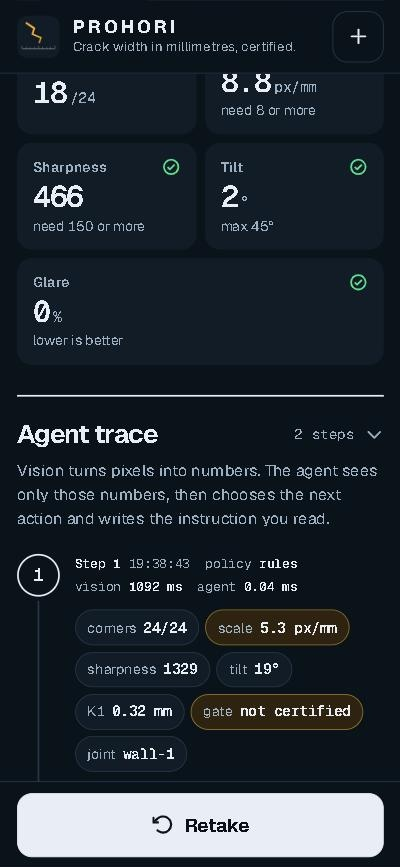
\includegraphics[width=0.235\textwidth]{img/crop_05_quality_and_agent_trace.jpg}
  \caption{The live phone app. Left to right: photo taken too far away (move closer); certified width after moving closer; all cracks and joint history; photo quality and agent trace.}
\end{figure}

\needspace{22\baselineskip}
\section{Data}
Field ground truth for crack width is hard to obtain, so we built our own test panel with known widths and supplemented it with public datasets.

\begin{center}
\small
\begin{tabularx}{\textwidth}{@{}>{\raggedright\arraybackslash}p{2.9cm}>{\raggedright\arraybackslash}X>{\raggedright\arraybackslash}p{2.4cm}>{\raggedright\arraybackslash}p{3.0cm}@{}}
\toprule
Dataset & Source & Size & Used for \\
\midrule
Ground-truth test panel & Our own. An A4 sheet with the ChArUco board (140$\times$100\,mm) and eight printed cracks of exact width (0.30, 0.40, 0.50, 0.75, 1.00, 1.50, 2.00, 3.00\,mm), generated by our script, printed at 100\% scale on matte paper and photographed with a 12\,MP smartphone on 19~Oct~2026 at varied distances and angles. & 29 photos, 168 crack measurements & Width accuracy (Fig.~1, results table) \\
\addlinespace
Degraded captures & Generated from the panel photos with controlled blur, motion blur, noise, JPEG compression, glare, extra tilt and lower resolution. & 2,584 captures, 18,683 measurements & Quality-gate calibration, 90\% ranges (Fig.~3) \\
\addlinespace
Simulated capture problems & Our capture simulator; its distance, tilt, blur and corner-count distributions are fitted to the real panel photos. & 100 held-out cases & Agent vs rules test (Fig.~4) \\
\addlinespace
krkCMd & Jakubowski \& Tomczak, \emph{Scientific Data} 12:165 (2025); Zenodo, CC~BY~4.0. High-resolution scans of real concrete cracks with operator-measured widths. & 19,098 width profiles & Resolution vs accuracy limits \\
\addlinespace
Public crack segmentation sets & Crack500, DeepCrack, TUT, CrackSeg9k, CFD, AEL, CrackTree200, GAPs384, Facade390, Road420, from the authors' official releases. & 10 datasets & Training the learned crack-segmentation model; real crack shapes for synthetic tests \\
\bottomrule
\end{tabularx}
\end{center}

\section{Results so far}
Width results are on the ground-truth panel photos; the agent result is on the simulated capture problems (Section~3):

\begin{center}
\begin{tabular}{lr}
\toprule
Average width error, certified cracks (held-out photos) & 0.048\,mm \\
True width inside the stated 90\% range (held-out photos) & 92.9\% \\
Capture agent recovery on multi-problem captures (vs fixed rules) & 85\% (62\%) \\
\bottomrule
\end{tabular}
\end{center}

\begin{figure}[H]
  \centering
  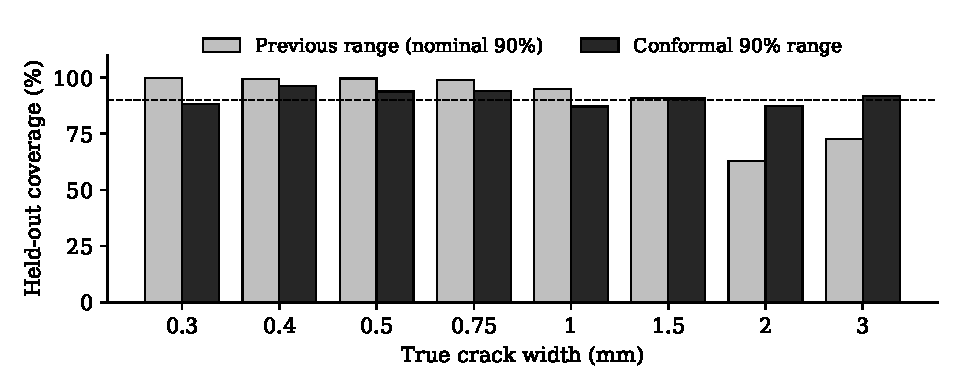
\includegraphics[width=0.82\textwidth]{img/coverage_bw.pdf}
  \caption{How often the stated 90\% range contains the true width, by crack width, on held-out data. The conformal range stays near 90\% at every width.}
\end{figure}

\begin{figure}[H]
  \centering
  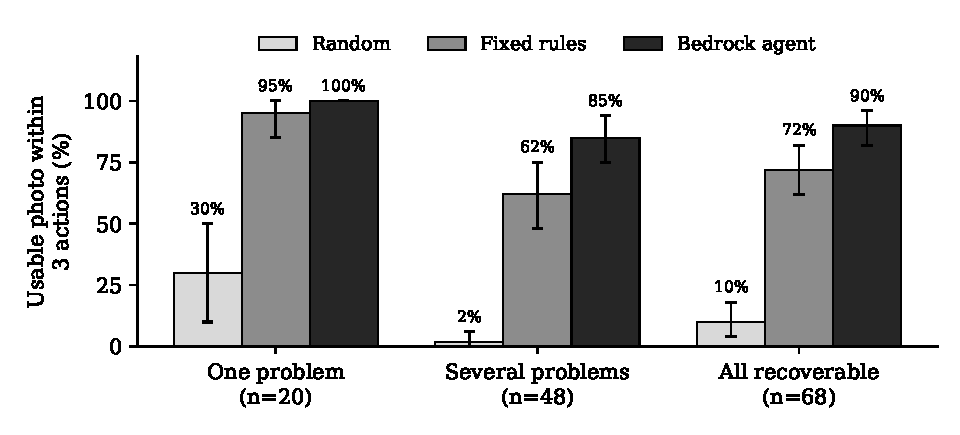
\includegraphics[width=0.82\textwidth]{img/agent_bw.pdf}
  \caption{Capture agent vs fixed rules on 100 held-out simulated capture problems (pre-registered test, 95\% confidence intervals).}
\end{figure}

\section{AWS usage}
Prohori runs as a production service in \texttt{us-east-1}:

\begin{figure}[H]
\centering
\resizebox{\textwidth}{!}{%
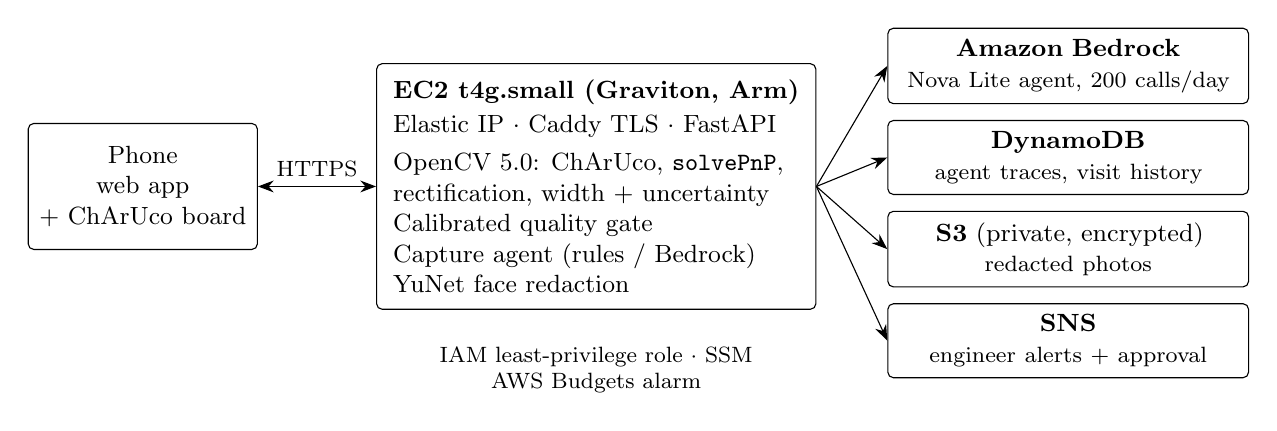
\begin{tikzpicture}[
  font=\small, >={Stealth[length=2mm]},
  box/.style={draw, rounded corners=2pt, align=center, inner sep=4pt},
  svc/.style={box, text width=4.3cm, minimum height=0.9cm}]
  \node[box, minimum height=1.6cm, minimum width=2.2cm] (phone) {Phone\\web app\\+ ChArUco board};
  \node[box, right=1.5cm of phone, align=left, inner sep=6pt] (ec2) {%
    \textbf{EC2 t4g.small (Graviton, Arm)}\\[1pt]
    Elastic IP $\cdot$ Caddy TLS $\cdot$ FastAPI\\[3pt]
    OpenCV 5.0: ChArUco, \texttt{solvePnP},\\
    rectification, width + uncertainty\\
    Calibrated quality gate\\
    Capture agent (rules / Bedrock)\\
    YuNet face redaction};
  \node[svc, right=0.9cm of ec2.north east, anchor=north west, yshift=0.45cm] (bed) {\textbf{Amazon Bedrock}\\ \footnotesize Nova Lite agent, 200 calls/day};
  \node[svc, below=0.2cm of bed] (ddb) {\textbf{DynamoDB}\\ \footnotesize agent traces, visit history};
  \node[svc, below=0.2cm of ddb] (s3) {\textbf{S3} (private, encrypted)\\ \footnotesize redacted photos};
  \node[svc, below=0.2cm of s3] (sns) {\textbf{SNS}\\ \footnotesize engineer alerts + approval};
  \draw[<->] (phone) -- node[above, font=\footnotesize]{HTTPS} (ec2);
  \foreach \t in {bed,ddb,s3,sns} \draw[->] (ec2.east) -- (\t.west);
  \node[below=0.35cm of ec2, font=\footnotesize, align=center] {IAM least-privilege role $\cdot$ SSM\\AWS Budgets alarm};
\end{tikzpicture}}
\caption{Prohori architecture on AWS (\texttt{us-east-1}).}
\end{figure}
\begin{itemize}
  \item \textbf{EC2 Graviton t4g.small} running OpenCV 5.0 behind HTTPS (Elastic IP, Caddy).
  \item \textbf{Amazon Bedrock} (Nova Lite) for the capture agent, capped at 200 calls per day.
  \item \textbf{DynamoDB} for agent traces and visit history; \textbf{S3} (private, encrypted) for photos.
  \item \textbf{SNS} for engineer alerts; \textbf{IAM}, \textbf{SSM} and an \textbf{AWS Budgets} alarm.
\end{itemize}

The service was built to run at low cost, so usage to date is covered by the account's Free Tier credits (\$120 remaining on 19 October); the full Bedrock agent evaluation cost \$0.06. The grant funds the final stage:

\begin{center}
\begin{tabularx}{0.92\textwidth}{Xr}
\toprule
Item & Estimate \\
\midrule
GPU training of a learned crack-segmentation model (EC2 GPU instance) & \$25 \\
Graviton4 (c8g) benchmark with the OpenCV COOL build (Paid plan) & \$20 \\
Hosting the live service through judging and a 3-month pilot & \$55 \\
Bedrock usage for evaluation, demo video and judging & \$10 \\
Storage, alerts and field-test traffic & \$40 \\
\midrule
\textbf{Total} & \textbf{\$150} \\
\bottomrule
\end{tabularx}
\end{center}

\section{Remaining work (to 26 October)}
\begin{center}
\begin{tabularx}{0.92\textwidth}{Xr}
\toprule
Deploy the calibrated quality gate and updated agent & 21 Oct \\
Train the learned crack-segmentation model & 23 Oct \\
Graviton4 + OpenCV COOL benchmark & 24 Oct \\
Improve thin-crack width accuracy & 24 Oct \\
Validation on real walls in Dhaka & 25 Oct \\
Write-up, demo video and submission & 26 Oct \\
\bottomrule
\end{tabularx}
\end{center}

Thank you for the grant and for the flexibility on the check-in.

\end{document}
